\chapter{Lec 03 - From DFS to BFS}

\section{More applications of DFS}
DFS can also be used to solve the following 2 problems:
\begin{itemize}
    \item Connected Components: Labelling all the vertices of $G$ such that 2 vertices have the same label iff they are in the same connected components.
    \item Connectivity: Return whether the graph is connected or not. 
\end{itemize}

\subsection{Connected Components}
\begin{algorithm}
\caption{ConnectedComponents}\label{Conn.Comp.}
    \begin{algorithmic}[1]
    \Procedure{ConnectedComp ($G$)}{}
        \For{$v \gets 1$ to $n$}
            \State $L_{V}[v].ID = 0$
        \EndFor
        \State $k \gets 0$
        \For{$v \gets 1$ to $n$}
            \If{$L_{V}[v].ID = 0$}
                \State $k \gets k + 1$
                \State DFS($G, v, k$)
            \EndIf
        \EndFor
    \EndProcedure
    \end{algorithmic}
\end{algorithm}
We have to modify the DFS algorithm in such a way that $L_{V}[v] \gets k$. The $ID$ field of each node is no more either 0 or 1, but it corresponds to the ID of the $k$-th connected component. 

\subsection{Connectivity}
\begin{algorithm}
\caption{Connectivity}\label{Connectivity}
    \begin{algorithmic}[1]
    \Procedure{Connectivity ($G$)}{}
        \For{$v \gets 1$ to $n$}
            \State $L_{V}[v].ID = 0$
        \EndFor
        \State $k \gets 0$
        \For{$v \gets 1$ to $n$}
            \If{$L_{V}[v].ID = 0$}
                \State $k \gets k + 1$
                \State DFS($G, v, k$)
            \EndIf
        \EndFor
        \State \textbf{if} $k = 1$ \textbf{return} $Yes$ \textbf{else} $False$
    \EndProcedure
    \end{algorithmic}
\end{algorithm}
The algorithm is similar to the one used for computing the connected components, but in this case we return if the graph is connected or not ($k = 1$).\newline\newline
The complexity of both algorithms is $\Theta(n + m)$.

\section{Summary}
Given a graph $G = (V, E)$, the following problems can be solved using DFS:
\begin{itemize}
    \item Test if $G$ is connected.
    \item Find the connected components of $G$.
    \item Find a spanning tree of $G$ (if $G$ is connected).
    \item Find a path between 2 vertices (if any).
    \item Find a cycle (if any).
\end{itemize}

\section{Breadth-First search (BFS)}
BFS is an \textbf{iterative} algorithm that, starting from a source vertex $s$, visits all the vertices in the same connected components of $s$, and it partitions all the vertices in levels $L_{i}$ depending on their distance $i$ from $s$. \newline\newline
As we did for DFS, every vertex $v$ has a field $L_{v}[v].ID$ which can either be 1 if the vertex has been visited, 0 otherwise. Furhermore, every edge $e$ has a field $L_{E}[e].Label$ which can either be null or \textit{Discovery edge / Cross edge}.
\begin{algorithm}
\caption{BFS}\label{BFS}
    \begin{algorithmic}[1]
    \Procedure{BFS ($G, s$)}{}
     \State visit(s)
     \State $L_{V}[s].ID = 1$
     \State Create a set $L_{0}$ containing $s$
     \State $i \gets 0$
     \While{! $L_{i}.isEmpty$}
        \State Create a set of vertices $L_{i+1}$
        \For{$v \in L_{i}$}
            \For{$e \in G.incidentEdges(v)$}
                \If{$L_{E}[e].label = null$}
                    \State $w \gets G.opposite(v, e)$
                    \If{$L_{V}[w].ID = 0$}
                        \State $L_{E}[e].label \gets \text{Discovery Edge}$
                        \State visit($w$)
                        \State $L_{V}[w].ID \gets 1$
                        \State add $w$ in $L_{i + 1}$
                    \Else
                        \State $L_{E}[e].label \gets \text{Cross Edge}$
                    \EndIf
                \EndIf
            \EndFor
        \EndFor
        \State $i \gets i + 1$
     \EndWhile
    \EndProcedure
    \end{algorithmic}
\end{algorithm}\newline\newline
\textbf{Example:}\newline\newline
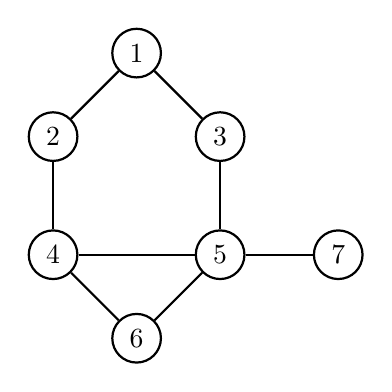
\begin{tikzpicture}[node distance={15mm}, thick, main/.style = {draw, circle}] 
            \node[main] (1) {$1$}; 
            \node[main] (2) [below left of=1] {$2$}; 
            \node[main] (3) [below right of=1] {$3$}; 
            \node[main] (4) [below of=2] {$4$}; 
            \node[main] (5) [below of=3] {$5$};
            \node[main] (6) [below right of=4] {$6$};
            \node[main] (7) [right of=5] {$7$};
            \draw (1) -- (2); 
            \draw (1) -- (3); 
            \draw (2) -- (4);
            \draw (3) -- (5);
            \draw (4) -- (5);
            \draw (4) -- (6);
            \draw (5) -- (6);
            \draw (5) -- (7);
\end{tikzpicture}\newline\newline
\textbf{DFS:} $1 \rightarrow 2 \rightarrow 3 \rightarrow 4 \rightarrow 5 \rightarrow 6 \rightarrow 7$
\begin{itemize}
    \item $L_{0} = \{1\}$
    \item $L_{1} = \{2, 3\}$
    \item $L_{2} = \{4, 5\}$
    \item $L_{3} = \{6, 7\}$
\end{itemize}

\subsection{Correctness}
At the end of BFS($G, s$) we have:
\begin{enumerate}
    \item All the vertices in $C_{s}$ are visited and all the edges are labelled \textit{Discovery Edges} or \textit{Cross Edges}

    \item The set of \textit{Discovery Edges} are a spanning tree $T$ of $C_{s}$ which is called BFS Tree.

    \item $\forall v \in L_{i}$ the path in $T$ from $s$ to $v$ has $i$ edges and every other path from $s$ to $v$ has at least $i$ edges (i.e. $\geq i$ edges)
\end{enumerate}
The proof of the first two properties is the same as for the DFS.\newline\newline
\textbf{Proof of 3:}\newline
Let $P: s = u_{0} \rightarrow u_{1} \rightarrow ... \rightarrow u_{i} = v$ a path from $s$ to $v$, where $u_{j} \in L_{j}$ is \textit{discovered} from the vertex $u_{j - 1} \forall j$. Then, the edge $(u_{j - 1}, u_{j})$ is a \textit{Discovery Edge}. By contradiction, assume assume $\exists$ a path $P': s = z_{0} \rightarrow z_{1} \rightarrow ... \rightarrow z_{t} = v$ with $t < i$. This implies that $ s = z_{0} \in L_{0}$, $z_{1} \in L_{1}$, $z_{2} \in L_{1} \,\, or \,\, L_{2}$, ..., $z_{t} \in L_{1} \,\, or \,\, L_{2} \,\, or \,\,...\,\,L_{t}$. This means that, since $z_{t} = v$, $v \notin L_{i}$, but this is a contradiction.

\subsection{Complexity}
$\forall v \in C_{s}$ there is one iteration of the first \textbf{for} loop and $d(v)$ iterations of the second \textbf{for} loop. Then, the complexity of BFS is:
\[\Theta\left( \sum_{v \in C_{s}} d(v)\right) = \Theta(m_{s})\]

\subsection{Applications}
\begin{itemize}
    \item Same as for DFS in $\Theta(n + m)$ time
    \item Given a graph $G = (V, E)$ and $s,t \in V$ return the \textbf{shortest} path from $s$ to $v$ (if any) \footnote{Shortest path in terms of number of edges between the two nodes}. In order to solve this problem, we can build the path following the same approach as for DFS.
\end{itemize}

